\chapter{النشاط البدني والصحة}\label{ch:g10:sport-and-health}

تلميذان في السادسة عشرة. أحدهما يمشي إلى المدرسة، ويلعب كرة السلة
مرتين في الأسبوع، وينام ثماني ساعات؛ والآخر يقلّ بالسيارة، ويقضي
المساء جالسًا أمام شاشة، وينام ستًا. وهما في السادسة عشرة متشابهان.
أما في الخمسين فسيرى طبيباهما شخصين مختلفين: الأول بقلب شخص أصغر منه
بعشرين سنة وعظامه وعضلاته وسكر دمه، والثاني بقائمة من الحالات تبدأ
بكلمة «مزمن». وقد بينت الفصول الثلاثة السابقة ما يفعله الجسم العامل؛
وهذا الفصل عما يفعله العمل المنتظم به --- وما ينقضه سوء الاستعمال، في
صورة إفراط في \omterm{def:g10:sport-and-health:training}{التدريب} أو منشطات.

\section{ما الذي يغيره التدريب}

\begin{definition}[النشاط البدني والتدريب]\label{def:g10:sport-and-health:training}
\emph{النشاط البدني}\index{نشاط بدني} كل حركة للجسم تنتجها العضلات
وترفع \omterm{def:g10:exercise-and-energy:expenditure}{الإنفاق الطاقي} فوق الراحة: مشيًا وصعود سلالم وأشغال بيت
ورياضة. أما \emph{التدريب} فنشاط بدني يكرر بقصد تحسين قدرة ما. ويستجيب
الجسم لطلب متكرر بأن \emph{يتكيف}: فيكبّر البنى التي يحمّلها الطلب أو
يقويها أو يعيد تجهيزها --- شرط أن تتلو الطلبَ الراحةُ التي يبنى فيها
التكيف.
\end{definition}

\begin{proposition}[التكيفات لتدريب التحمل]\label{prop:g10:sport-and-health:endurance}
الجهد المتكرر الطويل المدة المعتدل الشدة، على مدى أشهر، ينتج:
\begin{itemize}
  \item قلبًا أكبر وأقوى: فيرتفع الحجم النفضي، ويهبط تواتر الراحة (من
        70 إلى 50 أو دونها)، ويزيد الصبيب الأقصى و
        $\dot V\!\mathrm{O_2}$max بنسبة 10\% إلى 30\%؛
  \item شعيرات دموية أكثر ومتقدرات أكثر في \omterm{def:g10:muscles-and-joints:muscle}{الألياف العضلية}، فتحرق
        نصيبًا أكبر من الشحم وتنتج حمضًا لبنيًا أقل عند استطاعة معطاة؛
  \item كريات حمراء أكثر، ومنه أكسجين أكثر محمولًا في اللتر؛
  \item مخازن \omterm{def:g10:exercise-and-energy:glycogen}{غليكوجين} أكبر، وجسمًا ينظم سكر دمه وضغط دمه بيسر أكبر.
\end{itemize}
\end{proposition}
\admitted

\begin{omfigure}
\begin{tikzpicture}
\begin{axis}[
  width=0.86\linewidth, height=5.6cm,
  axis x line=bottom, axis y line=left,
  xmin=0, xmax=26, ymin=40, ymax=80,
  xlabel={أسابيع التدريب}, ylabel={تواتر القلب في الراحة (في الدقيقة)},
  xlabel style={font=\small, at={(axis description cs:0.5,-0.12)}, anchor=north},
  ylabel style={font=\small},
  tick label style={font=\small}, xtick={0,4,8,12,16,20,24}, ytick={40,50,60,70,80},
  legend style={at={(0.5,-0.3)}, anchor=north, legend columns=2, font=\small, draw=none},
]
\addplot[thick, omThm, mark=*, mark size=1.5pt] coordinates
  {(0,72) (4,68) (8,64) (12,60) (16,57) (20,55) (24,54)};
\addplot[thick, omDef, mark=square*, mark size=1.5pt] coordinates
  {(0,72) (4,70) (8,66) (12,64) (16,62) (20,61) (24,61)};
\legend{{4 حصص في الأسبوع}, {حصتان في الأسبوع}}
\end{axis}
\end{tikzpicture}

{\small تواتر القلب في الراحة عند مجموعتين من المبتدئين على مدى ستة
أشهر من الجري. والهبوط يعكس حجمًا نفضيًا متناميًا: أي \qty{5}{L/min}
نفسها في الراحة بنبضات أقل. والتكيف يتناسب مع الطلب، ويبطؤ كلما اقترب
الجسم من حاله الجديدة.}
\end{omfigure}

\begin{example}[أرقام التكيف]\label{ex:g10:sport-and-health:numbers}
شاب في السابعة عشرة قليل الحركة و$\dot V\!\mathrm{O_2}$max عنده
\qty{40}{mL/min} لكل كيلوغرام يجري ثلاث مرات في الأسبوع ستة أشهر:
فيصير \num{48}، ويهبط تواتر قلبه في الراحة من 72 إلى 58. وتبين خزعته
العضلية متقدرات أكثر بنسبة 40\% وشعيرات دموية أكثر بنسبة 30\% لكل
ليف. وألياف عضلاته هي هي عددًا وصنفًا؛ وإنما أعيد تجهيزها.
\end{example}

\begin{proposition}[التكيفات لتدريب القوة]\label{prop:g10:sport-and-health:strength}
الانقباضات المتكررة في مقابل أحمال ثقيلة تغلّظ \omterm{def:g10:muscles-and-joints:muscle}{الألياف العضلية}
(بلييفات أكثر في كل ليف) وتحسّن الأمر العصبي الذي يجندها؛ وتستطيع
القوة أن تتضاعف في سنة من دون أن يتغير عدد الألياف. وتغلظ كذلك
الأوتار والعظام التي يحمّلها \omterm{def:g10:sport-and-health:training}{التدريب}، لكن ببطء أشد. والعظم بخاصة يبنى
ويصان استجابة للأحمال التي يحملها: فالمراهقة النشطة تضبط كتلة العظم
التي ستسحب منها في الشيخوخة، والطرف المشلول في جبيرة يفقد عظمًا في
غضون أسابيع.
\end{proposition}
\admitted

\section{النشاط والصحة}

\begin{proposition}[آثار النشاط المنتظم في الصحة]\label{prop:g10:sport-and-health:health}
\omterm{def:g10:sport-and-health:training}{النشاط البدني} المنتظم --- بما يعادل ساعة في اليوم من نشاط معتدل
للمراهقين، ونصف ساعة للبالغين --- يخفض خطر أشيع الأمراض المزمنة: أمراض
القلب والشرايين، والسكري من النمط الثاني، وعدة سرطانات، وتخلخل العظام،
والاكتئاب. وهو يفعل ذلك بالتكيفات المذكورة أعلاه: قلب وأوعية تعمل
بضغط أدنى، وعضلات تسحب الغلوكوز من الدم بسهولة، وعظام تحفظ كتلتها،
وكتلة جسم تبقى في مدى صحي. والأثر كبير --- يضاهي أثر الامتناع عن
التدخين --- وهو لا يقتضي رياضة، بل حركة فحسب.
\end{proposition}
\begin{proof}[شواهد]
تجد دراسات تتابع عشرات الألوف من الناس عقودًا أن من هم في الخمس الأنشط
من السكان يموتون، عند عمر معطى، بنحو نصف نسبة من هم في الخمس الأقل
نشاطًا، ويفسر مرض القلب معظم الفرق؛ والعلاقة تصمد بعد مراعاة الغذاء
والتدخين والظروف الاجتماعية، وهي متدرجة --- فكل درجة صعود في النشاط
تجلب درجة هبوط في الخطر. والتجارب التي يوزَّع فيها أشخاص قليلو الحركة
على برنامج مشي تبين هبوطًا في ضغط الدم وسكر الدم في غضون أشهر.
\end{proof}

\begin{omfigure}
\begin{tikzpicture}
\begin{axis}[
  ybar, bar width=16pt,
  width=0.8\linewidth, height=5.4cm,
  axis x line=bottom, axis y line=left,
  ymin=0, ymax=1.2, ylabel={الخطر النسبي للوفاة},
  ylabel style={font=\small},
  symbolic x coords={الأقل نشاطًا, منخفض, معتدل, مرتفع, الأنشط},
  xtick=data, tick label style={font=\small},
  xlabel={أخماس السكان بحسب النشاط الأسبوعي},
  xlabel style={font=\small, at={(axis description cs:0.5,-0.14)}, anchor=north},
  enlarge x limits=0.15, ytick={0,0.2,0.4,0.6,0.8,1.0},
  nodes near coords, nodes near coords style={font=\scriptsize},
  every node near coord/.append style={/pgf/number format/fixed, /pgf/number format/precision=2},
]
\addplot[fill=omThm!50, draw=omThm] coordinates
  {(الأقل نشاطًا,1.00) (منخفض,0.80) (معتدل,0.70) (مرتفع,0.62) (الأنشط,0.55)};
\end{axis}
\end{tikzpicture}

{\small خطر الوفاة على مدى متابعة عشرين سنة، نسبةً إلى الخمس الأقل
نشاطًا، في جمهرة بالغة كبيرة (مقرَّبًا من عدة دراسات). كل درجة من
النشاط تخفض الخطر؛ وأكبر مكسب هو الأول، من لا شيء إلى شيء.}
\end{omfigure}

\begin{example}[سكر الدم والعضلة]\label{ex:g10:sport-and-health:sugar}
العضلة العاملة تأخذ الغلوكوز من الدم من دون حاجة إلى هرمون الأنسولين،
والعضلة المدرَّبة تبقى أشد حساسية للأنسولين بين الحصص. والمشي السريع
بعد وجبة يخفض ذروة غلوكوز الدم التي تتلوها؛ أما الجسم القليل الحركة،
إذا طلب منه تخزين السكر نفسه من دون حركة، فيحتاج إلى أنسولين أكثر كل
سنة --- وهو الطريق إلى السكري من النمط الثاني، وآليته موضوع السنة
الأخيرة.
\end{example}

\section{إفراط، وتسرع، وخطأ}

\begin{proposition}[الإفراط في التدريب والإصابة]\label{prop:g10:sport-and-health:overtraining}
التكيف يبنى أثناء الراحة. والطلب الذي يكرر بلا تعاف كافٍ --- حصص أكثر،
أو أثقل، مما تستطيع النسج إصلاحه بينها --- ينتج عكس التكيف: تعبًا
مستمرًا، وتواتر قلب في الراحة يرتفع، وأداءً يهبط، ونومًا مضطربًا،
وعدوى متكررة، وفي النسج الأبطأ إصلاحًا
(\cref{ch:g10:muscles-and-joints}) التهاب أوتار وكسور إجهاد. وأشيع
سبب للإصابة عند المراهقين ليس الرياضة بل النسبة التي يزاد بها حملها.
\end{proposition}
\admitted

\begin{example}[قاعدة العشرة بالمئة]\label{ex:g10:sport-and-health:tenpercent}
العدّاءة التي تزيد مسافتها الأسبوعية بما لا يتجاوز 10\% في الأسبوع
قلما تؤذي نفسها؛ أما التي تضاعفها في أسبوعين فكثيرًا ما تفعل. والعظم
\omterm{def:g10:muscles-and-joints:muscle}{والوتر} يتكيفان عبر أشهر، والعضلة والقلب عبر أسابيع: فالنسج البطيئة هي
التي تضبط النسبة التي يجوز أن يرتفع بها الحمل.
\end{example}

\begin{proposition}[المنشطات]\label{prop:g10:sport-and-health:doping}
\emph{المنشطات}\index{منشطات} هي استعمال مواد أو طرق ترفع الأداء
بالتأثير في تنظيم الجسم، بدل التكيف الذي كان \omterm{def:g10:sport-and-health:training}{التدريب} ليبنيه. وكل منها
يحاكي تكيفًا ويحمل كلفة الالتفاف عليه:
\begin{itemize}
  \item هرمون الإريثروبويتين (EPO)، أو نقل دم المرء نفسه المخزون،
        يرفع عدد الكريات الحمراء --- ويغلّظ الدم حتى يتخثر في أوعية
        القلب أو الدماغ؛
  \item الستيروئيدات البانية، المشتقة من التستوستيرون، تغلّظ \omterm{def:g10:muscles-and-joints:muscle}{الألياف
        العضلية} --- وتضطرب بها هرمونات الجسم نفسها والكبد والقلب
        والمزاج؛
  \item المنبهات تحجب التعب --- وتزيل الإنذار الذي يحمي القلب من فرط
        الحرارة والإنهاك؛
  \item هرمون النمو، والأدوية التي تخفي غيرها، تكمل القائمة.
\end{itemize}
\omterm{prop:g10:sport-and-health:doping}{والمنشطات} محرمة في المنافسة لأنها ظلم؛ وهي خطرة لأن كل مادة منها تلغي
تنظيمًا موجودًا لسبب.
\end{proposition}
\admitted

\begin{example}[EPO بالأرقام]\label{ex:g10:sport-and-health:epo}
تمثل الكريات الحمراء نحو 45\% من حجم الدم الطبيعي. وقد دفع تعاطي EPO
رياضيين إلى 55\% وأكثر، أي دم من الغلظ بحيث لا يستطيع القلب، وقد
أبطأه النوم، أن يحركه: فمات عدة دراجين شبان في نومهم في السنوات التي
سبقت وجود الاختبارات. أما \omterm{def:g10:sport-and-health:training}{التدريب} في الارتفاعات فيرفع الرقم نفسه
نقطتين أو ثلاثًا، عبر أسابيع، تحت سيطرة الجسم نفسه.
\end{example}

\section{قواعد كل يوم}

\begin{method}[التدريب بأمان]\label{met:g10:sport-and-health:rules}
\begin{enumerate}
  \item \emph{تقدّم ببطء}: زد الحمل نحو عشره في الأسبوع، ودع العظم
        \omterm{def:g10:muscles-and-joints:muscle}{والوتر} يضبطان الوتيرة.
  \item \emph{أحمِ وبرّد}: عشر دقائق لكل منهما، للأسباب المذكورة في
        \cref{ch:g10:muscles-and-joints}.
  \item \emph{اشرب}: ساعة من الجهد الشاق تفقد لترًا إلى لترين من
        العرق؛ فعوّضهما، مع بعض الملح، قبل أن يقول العطش ذلك --- ففقد
        2\% من كتلة الجسم يخفض الأداء من قبل.
  \item \emph{كُل للجهد}: \omterm{def:g10:chemistry-of-life:families}{كربوهيدرات} قبل الجهود الطويلة وأثناءها،
        وبروتينات للإصلاح بعدها
        (\cref{ch:g10:exercise-and-energy})؛ وما من مكمّل يحل محل
        غذاء متنوع.
  \item \emph{استرح}: النوم هو حين يبنى التكيف؛ وارتفاع تواتر القلب
        في الراحة أبكر علامة على قلته.
  \item \emph{أصغِ إلى الألم}: الألم الحاد في \omterm{def:g10:muscles-and-joints:joint}{مفصل} أو \omterm{def:g10:muscles-and-joints:muscle}{وتر} إشارة، لا
        عقبة.
\end{enumerate}
\end{method}

\begin{omfigure}
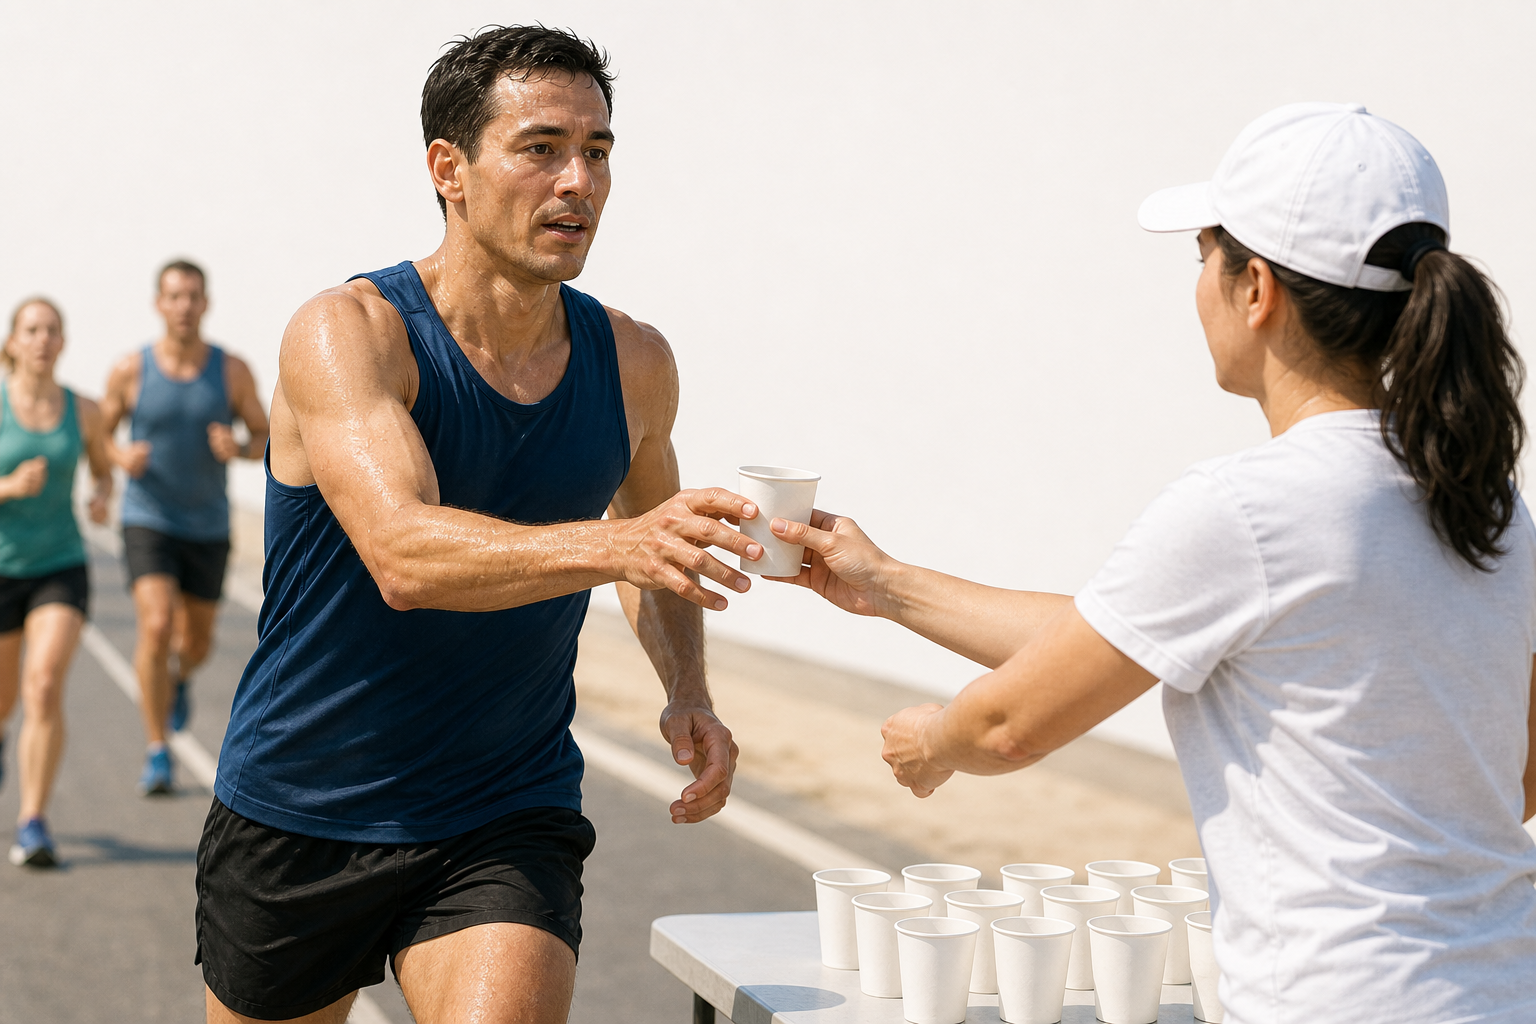
\includegraphics[width=0.62\linewidth]{images/book2/ai/g10-health-hydration.png}

{\small نقطة إمداد على مسار ماراثون. فعند نسبة تعرق تفوق لترًا في
الساعة، يجب تعويض الماء المفقود أثناء الجهد؛ وانتظار العطش يعني الجري
وقد بدأ التجفاف من قبل.}
\end{omfigure}

\begin{example}[الإماهة بالأرقام]\label{ex:g10:sport-and-health:water}
عدّاءة كتلتها \qty{60}{kg} تتعرق \qty{1.2}{L} في الساعة في طقس دافئ.
ففي جري ساعتين تفقد \qty{2.4}{kg}، أي 4\% من كتلتها: فيهبط حجم دمها،
ويرتفع تواتر قلبها عشر نبضات ليحفظ الصبيب، وتتسلق حرارة جسمها، وتهبط
وتيرتها العشر. ولو شربت نصف لتر في الساعة لخفضت الفقد إلى النصف.
\end{example}

\begin{remark}[الجسم يحفظ الحساب]\label{rem:g10:sport-and-health:account}
كل تكيف في هذا الفصل بنية يبنيها الجسم استجابة للاستعمال، وكل منها
يفكك من جديد حين يتوقف الاستعمال: فشهر في الفراش يفقد خمس العضلة، وسنة
من الخمول تفقد معظم مكاسب التحمل. والحساب يحفظ باستمرار، والرصيد في
الخمسين هو مجموع الإيداعات التي جرت في السادسة عشرة والسادسة والعشرين
والسادسة والثلاثين.
\end{remark}

\section{تمارين}

\begin{exercise}[$\star$]\label{exo:g10:sport-and-health:1}
اذكر أربعة تكيفات للجسم مع تدريب التحمل.
\end{exercise}

\begin{exercise}[$\star$]\label{exo:g10:sport-and-health:2}
لماذا يهبط تواتر القلب في الراحة \omterm{def:g10:sport-and-health:training}{بالتدريب}، مع أن \omterm{def:g10:heart-lungs-effort:output}{الصبيب القلبي} في
الراحة لا يتغير؟
\end{exercise}

\begin{exercise}[$\star$]\label{exo:g10:sport-and-health:3}
ما المقدار اليومي الموصى به من \omterm{def:g10:sport-and-health:training}{النشاط البدني} للمراهق؟ وهل يجب أن يكون
رياضة؟
\end{exercise}

\begin{exercise}[$\star$]\label{exo:g10:sport-and-health:4}
عرّف \omterm{prop:g10:sport-and-health:doping}{المنشطات} وأعطِ مثالين مع التنظيم الذي يلغيه كل منهما.
\end{exercise}

\begin{exercise}[$\star$]\label{exo:g10:sport-and-health:5}
سمِّ ثلاث علامات على الإفراط في \omterm{def:g10:sport-and-health:training}{التدريب}.
\end{exercise}

\begin{exercise}[$\star\star$]\label{exo:g10:sport-and-health:6}
من شكل تواتر القلب، قارن الهبوط بعد 12 أسبوعًا في المجموعتين، وقل ما
الذي يبينه ذلك عن العلاقة بين الطلب والتكيف.
\end{exercise}

\begin{exercise}[$\star\star$]\label{exo:g10:sport-and-health:7}
صبيب عدّاءة في الراحة \qty{5.0}{L/min}. ويهبط تواتر قلبها في الراحة
من 72 إلى 54 في ستة أشهر. فبأي عامل تغير حجمها النفضي؟
\end{exercise}

\begin{exercise}[$\star\star$]\label{exo:g10:sport-and-health:8}
من شكل الخطر النسبي، بأي نسبة يقل خطر الوفاة في الخمس الأنشط عنه في
الخمس الأقل نشاطًا؟ وأي درجة واحدة تجلب أكبر مكسب؟
\end{exercise}

\begin{exercise}[$\star\star$]\label{exo:g10:sport-and-health:9}
تلميذة كتلتها \qty{55}{kg} تلعب مباراة تنس ساعتين في الصيف، وتتعرق
\qty{1.0}{L} في الساعة ولا تشرب شيئًا. فأي نسبة من كتلتها فقدت، وما
ثلاث نتائج لذلك؟
\end{exercise}

\begin{exercise}[$\star\star$]\label{exo:g10:sport-and-health:10}
مبتدئ يجري \qty{10}{km} في الأسبوع. فباتباع قاعدة العشرة بالمئة، كم
أسبوعًا يلزم ليبلغ \qty{20}{km} في الأسبوع؟ (احسب أسبوعًا أسبوعًا، أو
لاحظ أن $1.1^7 \approx 1.95$.)
\end{exercise}

\begin{exercise}[$\star\star$]\label{exo:g10:sport-and-health:11}
فسّر لماذا تستطيع قوة العضلة أن تتضاعف في سنة من \omterm{def:g10:sport-and-health:training}{التدريب} بينما يبقى
عدد \omterm{def:g10:muscles-and-joints:muscle}{الألياف العضلية} كما هو.
\end{exercise}

\begin{exercise}[$\star\star\star$]\label{exo:g10:sport-and-health:12}
دم رياضي فيه 45\% كريات حمراء؛ وبعد تعاطي EPO، 56\%. باستعمال
\cref{ch:g10:heart-lungs-effort}، قدّر المكسب في الأكسجين المحمول لكل
لتر ومنه في $\dot V\!\mathrm{O_2}$max، وفسّر لماذا يشترى ذلك المكسب
بخطر خثرة قاتلة.
\end{exercise}

\begin{exercise}[$\star\star\star$]\label{exo:g10:sport-and-health:13}
\omterm{def:g10:sport-and-health:training}{التدريب} في الارتفاعات ثلاثة أسابيع يرفع الكريات الحمراء من 45\% إلى
48\%؛ وEPO يرفعها إلى 56\% في المدة نفسها. فبأي معنى يكون الأول تكيفًا
والثاني لا، مع أن الجزيء المعني واحد؟
\end{exercise}

\begin{exercise}[$\star\star\star$]\label{exo:g10:sport-and-health:14}
فسّر، باستعمال \cref{ex:g10:sport-and-health:sugar}، لماذا يصف
الأطباء المشي لمرضى بدأ سكر دمهم يرتفع، ولماذا تنفع تلك الوصفة أكثر
من دواء لا يفعل إلا خفض السكر.
\end{exercise}

\begin{exercise}[$\star\star\star$]\label{exo:g10:sport-and-health:15}
«شهر من \omterm{def:g10:sport-and-health:training}{التدريب} المكثف قبل موسم الامتحانات سيهيئني للسنة كلها.» ناقش
بمفاهيم التكيف والراحة وسلالم الزمن عند النسج المختلفة.
\end{exercise}

\section{مسألة: تلميذان، ثلاثون سنة}

\begin{problem}[{مسألة نهاية الأسبوع --- ابن ستة عشر نشط وآخر قليل
الحركة يتابعان عبر التدريب، وموسم من الإفراط في التدريب، والحسابات
التي يحفظها جسماهما إلى منتصف العمر}]
\label{pb:g10:sport-and-health:1}
أليكس وسام في السادسة عشرة، وكلاهما \qty{62}{kg}، وتواتر قلب في الراحة
72، و$\dot V\!\mathrm{O_2}$max \qty{42}{mL/min} لكل كيلوغرام. يبدأ
أليكس الجري ثلاث مرات في الأسبوع؛ وسام لا يبدأ.

\medskip
\noindent\textbf{الجزء الأول --- أليكس يتدرب.}
بعد ستة أشهر صار تواتر قلب أليكس في الراحة 56 و$\dot V\!\mathrm{O_2}$max
عنده \qty{50}{mL/min} لكل كيلوغرام؛ ولم يتغير تواتر قلبه الأقصى (200).
\begin{enumerate}
  \item صبيبه القلبي في الراحة لا يزال \qty{4.8}{L/min}. احسب حجمه
        النفضي قبل وبعد.
  \item احسب $\dot V\!\mathrm{O_2}$max عنده باللترات في الدقيقة قبل
        وبعد، والمكسب بالنسبة المئوية.
  \item بافتراض أن استخلاصه الأقصى للأكسجين (\qty{150}{mL} لكل لتر) لم
        يتغير، احسب صبيبه القلبي الأقصى قبل وبعد، وحجمه النفضي الأقصى
        قبل وبعد.
  \item أي تكيفات \cref{prop:g10:sport-and-health:endurance} يفسر
        المكسب في الحجم النفضي، وأيها يفسر مكسبًا في الاستخلاص؟
  \item انتقلت مسافة أليكس الأسبوعية من \qty{6}{km} إلى \qty{24}{km}
        في ستة أشهر. فهل احترمت قاعدة العشرة بالمئة؟ بيّن الحساب.
\end{enumerate}

\medskip
\noindent\textbf{الجزء الثاني --- أليكس يفرط في \omterm{def:g10:sport-and-health:training}{التدريب}.}
في الربيع يضاعف أليكس مسافته في أسبوعين استعدادًا لسباق. وبعد ثلاثة
أسابيع: تواتر قلب في الراحة 64، ونوم رديء، ونزلة برد، وألم في الساق،
وأزمنة سباق أبطأ.
\begin{enumerate}[resume]
  \item سمِّ الحالة واسرد العلامات الموافقة من الفصل.
  \item ما أرجح سبب لألم الساق، بمفردات
        \cref{ch:g10:muscles-and-joints}، ولماذا ذلك النسيج؟
  \item لماذا يرتفع تواتر القلب في الراحة، وقد كان \omterm{def:g10:sport-and-health:training}{التدريب} قد خفضه؟
  \item اقترح خطة لثلاثة أسابيع وعلّل كل عنصر فيها
        بالاعتماد على \cref{met:g10:sport-and-health:rules}.
  \item يعرض عليه زميل «مكمّلًا» يزيل التعب. فإلى أي صنف من
        \cref{prop:g10:sport-and-health:doping} ينتمي، وأي تنظيم
        يلغيه؟
\end{enumerate}

\medskip
\noindent\textbf{الجزء الثالث --- سام يجلس.}
في الثلاثين صار سام \qty{80}{kg}، وتواتر قلبه في الراحة 78 و
$\dot V\!\mathrm{O_2}$max عنده \qty{32}{mL/min} لكل كيلوغرام؛ أما
أليكس، وهو لا يزال نشطًا، فكتلته \qty{64}{kg} وتواتره 54 وقيمته \num{48}.
\begin{enumerate}[resume]
  \item احسب $\dot V\!\mathrm{O_2}$max عند الرجلين باللترات في
        الدقيقة. أي القيمتين المطلقتين أكبر، ولماذا كان الرقم لكل
        كيلوغرام هو المهم في الحياة اليومية؟
  \item صعود أربع درجات من السلالم يكلف كلًا منهما نحو \qty{12}{mL} من
        الأكسجين لكل كيلوغرام في الدقيقة فوق الراحة. فأي نسبة من حده
        الأقصى يستعمل كل منهما؟ ومن يصل لاهثًا؟
  \item يجد طبيب سام أن سكر دمه أعلى قليلًا من الطبيعي. فسّر، بالاعتماد على
        \cref{ex:g10:sport-and-health:sugar}، صلة ذلك بخموله.
  \item يصف له الطبيب نصف ساعة من المشي السريع في اليوم. باستعمال شكل
        الخطر النسبي، قدّر انخفاض الخطر على المدى البعيد إذا انتقل سام
        من الخمس الأقل نشاطًا إلى الخمس المعتدل.
  \item يعترض سام بأنه لا وقت لديه للرياضة. أجبه بالاعتماد على
        \cref{def:g10:sport-and-health:training}.
\end{enumerate}

\medskip
\noindent\textbf{الجزء الرابع --- الحساب في الخمسين.}
\begin{enumerate}[resume]
  \item تبلغ كتلة العظم ذروتها قرب الخامسة والعشرين ثم تتناقص نحو
        1\% في السنة. فإذا كانت ذروة أليكس أعلى 10\% من ذروة سام بسبب
        مراهقته النشطة، فكم سنة من التناقص يمثل ذلك الهامش؟
  \item بعد سقوط في الخمسين، يكسر سام رسغه ولا يكسره أليكس. اربط ذلك
        بالسؤال 16 وبما جاء في \cref{prop:g10:sport-and-health:strength}.
  \item انقطع أليكس عن \omterm{def:g10:sport-and-health:training}{التدريب} سنة في الأربعين بعد إصابة ففقد معظم
        مكاسب تحمله، ثم أعاد بناءها. فما الذي يبينه ذلك عن طبيعة
        التكيف؟
  \item اسرد، لسام في الخمسين، ثلاث حالات من
        \cref{prop:g10:sport-and-health:health} جعلها خموله أرجح،
        وآلية واحدة منها.
  \item اذكر النتيجة: الرقمان (تواتر القلب في الراحة،
        و$\dot V\!\mathrm{O_2}$max لكل كيلوغرام) اللذان يفصلان بين
        الرجلين في الثلاثين، والعادة الواحدة، مذكورةً بالساعات في
        الأسبوع، التي أنتجت الفرق.
\end{enumerate}
\end{problem}
